\documentclass[a4paper,10pt]{article}

\usepackage[T1]{fontenc}
\usepackage[utf8]{inputenc}
\usepackage[english]{babel}
\usepackage{natbib}
% \setcitestyle{authoryear,open={((},close={))}}

\usepackage{amsmath}
\usepackage{amssymb}

\usepackage{xcolor}
\usepackage{graphicx}
\usepackage{grffile}

\usepackage{subcaption}

\usepackage{booktabs}

\title{Bayesian Sparsification of $\cplx$-valued networks}
\author{Ivan Nazarov, and Evgeny Burnaev}

%% notation
\newcommand{\real}{\mathbb{R}}
\newcommand{\cplx}{\mathbb{C}}
\newcommand{\tr}[1]{\mathop{tr}{#1}}

\newcommand{\hop}{{\mkern-1.5mu\dagger}}
\newcommand{\conj}[1]{\overline{#1}}

% \renewcommand{\top}{{\mkern-1.5mu\intercal}}
\renewcommand{\vec}[1]{\overrightarrow{#1}}
\newcommand{\diag}[1]{\mathrm{diag}{#1}}

%% drafting macro
\newcommand{\important}[1]{\textbf{\!\colorbox{red}{#1}\!}}
\newcommand{\attn}[2]{\textbf{\color{red} #2~\textsuperscript{\textit{[#1]}}}}
\newcommand{\verify}[1]{\textit{\!\colorbox{red}{#1}\!}}
\newcommand{\rewrite}[1]{\attn{rewrite}{#1}}
\newcommand{\todo}[1]{{\color{blue} [TODO]} \important{#1}}

%% red-highlight missing citations
\usepackage{etoolbox}
\makeatletter
\patchcmd{\@citex}{\bfseries ?}{\colorbox{red}{\bfseries ?}}{}{}
\makeatother

\begin{document}
\maketitle

\section{Introduction} % (fold)
\label{sec:introduction}

% general intro text with motivation
Deep neural networks are an integral part of machine learning and data science toolset
for practical data-driven problem solving. With continual miniaturization ever more
applications can be found in embeded systems. Common embedded applications include
on-device image recognition and signal processing. Despite recent advances in generalization
and optimization theory specific to deep networks, deploying in actual embedded hardware
remains a challenge due to storage, real-time throughput, and numerical computational
compelexity restrictions.

These applications establish a need for sparsification and model compression techniques.
However audio or radio frequiency signal analysis is inherently complex-valued, yet
$\cplx$-valued models and neural networks and, in particular, comprssion methods tailored
to $\cplx$-networks remain a niche field of research. Although computational efficiency
reduction methods such as quantization and integer-based arithmetic appear to be directly
transferrable to $\cplx$-field, \citep{citation_needed}, the most promising methods,
\citep{gale_state_2019} such as weight pruning \citep{zuo_compression_2019}, bayesian 
dropout \citep{kingma_variational_2015}, and \citep{louizos_learning_2017} require
additional considerations.


% on sparsification
Solving the storage and compute constraints encourages development of model compression
and sparsification methods, that focus on favourable tradeoff between performance and size.
%
Most popular techniques include
model quantization from IEEE754,
and dropout. The key assumption is that the more explicitly zero parameters there is,
the less computations is needed.


\citet{monning_evaluation_2018} state,
that $\cplx$-networks have less intuitive architectures, inherently higher numerical
complexity due to multiplication in $\cplx$, that requires 3-4 floating point multiplications,
dependening on the implementation.


% due to them not being true cplx and just paired real computational graphs


% on dropout
Dropout, \citep{hinton_improving_2012}, prevents overfitting by injecting multiplicative
binary noise into layer's weights, thereby breaking up co-adaptations that could occur
during training. \citet{wang_fast_2013} argue that the overall effect of binary dropout
on the intermediate outputs via the Central Limit Theorem can be approximated by a Gaussian
with weight-input dependent mean and variance. \citet{srivastava_dropout_2014} propse
using independent $\mathcal{N}(1,1)$ noise, arguing that higher entroy of a Gaussian has
better regularizing effect. In multitask learning \citet{cheung_superposition_2019}
has shown the possiblity of storing task-specific parameters in non-destructive superposition
within a single network. Their argument implies that if the single task setting is viewed
as replicated mutlitask learning, then by sampling uncorrelated weight masks dropout acts
as superposition method, which better utilizes the learnig capacity of the network.
% many identical copies of the same task; \cite[Appendix A.1]{cheung_superposition_2019}

% segue into bayesian inference
Dropout resembles averaging models with shared parameters: each model is weighted equally
since masks are randomly sampled, unlike bayesian model averaging, which weighs accoring to
the posterior distribution. \citet{kingma_variational_2015} specifically consider dropout
as a Bayesian inference technique. Bayesian Inference as a principled framework of reasoning
about uncertainty, updates prior beliefs in accordance with the likelihood of empirical
observations into posterior belief. Under suitable modelling and prior assumptions, Bayesian
methods can be used towards model sparsification, \citep{kingma_variational_2015,molchanov_variational_2017},
and \citep{kharitonov_variational_2018}.

% out contribution
Inspired by variational sparsification techniques we develop bayesian dropout for $\cplx$-vlaued
networks.



\citep{yang_complex_2019,monning_evaluation_2018}

% complex nets and related stuff
data that is naturally complex-valued
studies have shown a potentially richer representation of complex nets
\citep{hirose2003,fijulamin2009}
% [3] Akira Hirose, Complex-valued neural networks: theories and applications, vol. 5, World Scientific, 2003.
% [4] Md Faijul Amin and Kazuyuki Murase, “Single-layered complex-valued neural network for real-valued classification problems,” Neurocomputing, vol. 72, no. 4-6, pp. 945–955, 2009.

the complex version of backpropagation algorithm  was proposed because of
its richer representational capacity.
% Nevio Benvenuto and Francesco Piazza, “On the complex backpropagation algorithm,” IEEE Transactions on Signal Processing, vol. 40, no. 4, pp. 967–969, 1992.


\citep{yang_complex_2019} develop complex transformer, with $\cplx$-attention and complex
encoder-decoder, and apply it to music transcription and wireless signal classification.

that interfaces the rest of
$\cplx$-valued
the network with complex numbers


that operates on the Fourier transform input speech, acoustic, of radio signals.

papers related to complex-valued distributions \citep{pav_moments_2015,taubock_complex-valued_2012},
and \citep{karseras_caution:_2014}

Application of complex-valued networks is not new, \citep{citation_needed}. More recently
they were applied to music transcription and speech recognition \citep{trabelsi_deep_2017},
and \citep{yang_complex_2019}. The key motivation behind adoption of $\cplx$-networks is
pervasiveness of $\cplx$-valued data in digital signal processing \citep{citation_needed},
acoustic and radio signal analysis \citep{citation_needed}, and quantum systems modelling
\citep{citation_needed}, etc. All these applications require compliance with algebraic
operations in the field of complex numbers.



The paper is structured as follows. In sec.~\ref{sec:bayesian_dropout} we review Bayesian
dropout techniques, and ins sec.~\ref{sec:c_valued_networks} we provide a brief summary of
the inner working of complex-valued networks as functions of complex argument. The main
contribution of this study is presented in sec.~\ref{sec:dropout_for_c_valued_layers},
where we consider different variational approximations and priors, outline the tricks
and derive expressions for the divergence term. In sec.~\ref{sec:experiments} we evaluate
the sparsification rate and compare the resulting performance of various $\cplx$-networks
proposed in prior work, and discuss the outcomes in sec.~\ref{sec:discussion_and_related_research}.

% section introduction (end)


\section{Bayesian Dropout} % (fold)
\label{sec:bayesian_dropout}

In general, the core of Bayesian Inference can be summarized as follows: given a prior
distribution $\pi(m)$ on models (hypotheses) $\mathcal{M}$, utilize the empirical evidence
$D$ to update the assumptions by considering the likelihood of the observations under each
$m \in \mathcal{M}$. Models are represented by a parametric family indexed by $\omega \in
\Omega$ and each $m_\omega(\cdot)$ specifies the conditional distribution of the data $
  D = (z_i)_{i=1}^N
$. The posterior distribution $p(\omega \mid D)$, derived using the Bayes rule $
  p(m \mid D) = \tfrac{p(D \mid m) \pi(m)}{p(D)}
$ with $
  p(D) = \mathbb{E}_{\pi(m)} p(D \mid m)
$, provides useful information about yet unobserved data and model parameters, e.g
classification uncertainty, predictive statistics, and parameter relevance.

The posterior itself is computationally intractable, save for the relatively simple cases
\citep{citation_needed}, and therefore exact inference is traded for tractability and scalability
of Variational Inference. Instead of deriving $p(\omega \mid D)$ using the rule, this approach
recasts posterior inference into variational optimization problem: finding $q$ that is close
to $p(\omega \mid D)$ in terms of a proximity score $\rho$
\begin{equation}  \label{eq:variational-progam}
  q_*
    \in \arg \min_{\theta} \rho\bigl(
      q_\theta(\omega), p(\omega \mid D)
    \bigr)
    \,,
\end{equation}
over a tractable parametric family of distributions on the parameter space $
  \mathcal{Q} = \{Q_\theta(d\omega) \colon \theta \in \Theta\}
$, $\theta$ -- generic variational parameter. The class $\mathcal{Q}$ is picked so that
its members have tractable densities $
  q_\theta(\omega) d\omega
$, can be sampled from and possess tractable $\log$-derivatives $
  \omega \mapsto \nabla_\theta \log q_\theta(\omega)
$, \citep{williams_simple_1992}, or can be represented as differentiable transformations
of non-parametric noise, \citep{kingma_auto-encoding_2014,figurnov_implicit_2019}.
% (reparameterization trick, pathwise gradieent) $q_{\theta}(d\omega)$ is a push-forward
% of $p(d\varepsilon)$ by a differentiable map $g(\varepsilon; \theta)$.
% % http://stillbreeze.github.io/REINFORCE-vs-Reparameterization-trick/#fn:1

Kullback-Leibler divergence of density $q$ from $p$ is
\begin{equation}  \label{eq:kl-div-def}
  KL(q \| p)
    % = \int \frac{dQ}{dP} \log{\frac{dQ}{dP}} P(d\omega)
    % = \int \frac{q(\omega)}{p(\omega)} \log{\frac{q(\omega)}{p(\omega)}} p(\omega) d\omega
    % = \mathbb{E}_{\omega \sim q}
    %   \log\frac{q(\omega)}{p(\omega)}
    = \mathbb{E}_{\omega \sim q}
      \log{q(\omega)}
    - \mathbb{E}_{\omega \sim q}
      \log{p(\omega)}
    \,,
\end{equation}
% and, despite it not being a metric and requiring distributions with nested support,
and is the natural choice for $\rho$, the main reason being that it satisfies the following
identity for well-behaved densities:
\begin{multline}  \label{eq:kl-div-master}
  % \log p(D)
    % = \mathbb{E}_{q(\omega)} \log \frac{p(D, \omega)}{p(\omega \mid D)}
    % = \mathbb{E}_{q(\omega)} \log \frac{
    %   p(D \mid \omega) \pi(\omega)
    % }{p(\omega \mid D)}
    % = \mathbb{E}_{q(\omega)} \log \frac{
    %   p(D \mid \omega) \pi(\omega)
    % }{q(\omega)}
    % + \mathbb{E}_{q(\omega)} \log \frac{q(\omega)}{p(\omega \mid D)}
    % - \mathbb{E}_{q(\omega)} \log \frac{q(\omega)}{\pi(\omega)}
    % = \mathbb{E}_{q(\omega)} \log{p(D \mid \omega)}
    % + \mathbb{E}_{q(\omega)} \log \frac{q(\omega)}{p(\omega \mid D)}
  \log p(D)
    - KL(q \| p(\omega \mid D))
    \\ = \mathbb{E}_{q(\omega)} \log{p(D \mid \omega)}
    - KL(q \| \pi)
    \,.
\end{multline}
This identity yields an equivalent problem for \eqref{eq:variational-progam}:
maximizing the \textit{evidence lower bound} (ELBO)
\begin{equation}  \label{eq:elbo_general}
  \mathcal{L}(\theta; \phi, \lambda)
    = - KL(q_{\theta} \| \pi_{\lambda})
      + \mathbb{E}_{\omega \sim q_{\theta}}
        \log p_{\phi}(D \mid \omega)
      % \mathbb{E}_{\omega \sim q_{\theta}}
        % \log\frac{q_\theta(\omega)}{\pi_{\lambda}(\omega)}
  % = \mathbb{E}_{\omega \sim q_{\theta}}
  %     \log{p_{\phi}(D \mid \omega) \pi_{\lambda}(\omega)}
  %   + \mathbb{H}(q_{\theta})
  \,,
\end{equation}
where the prior and likelihood are allowed to depend on explicit parameters. The most
commonly used algorithm to optimize \eqref{eq:elbo_general} is EM-algorithm. Other
variational objectives are possible, provided $p(\omega \mid D)$ is probed only through
$\log p(D \mid \omega)$ and $\log \pi(\omega)$, \citep{ranganath_operator_2018}.

\textit{Stochastic Gradient Variational Bayes} (SGVB), proposed by \citep{kingma_auto-encoding_2014},
is a differentiable unbiased Monte-Carlo estimator of \eqref{eq:elbo_general}, which makes
it possible to employ stochastic gradient-based optimization methods. If $
  \omega \sim q_{\theta}
$ is equivalent in distribution to $
  \omega = g(\varepsilon; \theta)
$ for some non-parametric random variable $
    \varepsilon \sim p_\varepsilon
$ and differentiable $
  g(\varepsilon; \theta)
$, then the SGVB is
\begin{equation}  \label{eq:sgvb}
  \widetilde{\mathcal{L}}(\theta; \phi, \lambda)
    = - KL(q_{\theta} \| \pi_{\lambda})
      % + \frac{N}{\lvert B \rvert} \sum_{i\in B}
        % \log p(z_i \mid \omega_i)b
      + \frac1{L} \sum_{l=1}^L
        \log p_{\phi}(D \mid g(\varepsilon_{l}; \theta))
        % \log p_{\phi}(D \mid \omega_{l})
        %   \Big\vert_{\omega_{l} = g(\varepsilon_{l}; \theta)}
      % =
      % - KL(q_{\theta} \| \pi)
      % + N \mathbb{E}_{B \sim \{D\}_M \otimes q_\theta^M}
        % \hat{\mathbb{E}}_{z,\omega \sim B}
          % \log p(z \mid \omega)
    \,, 
\end{equation}
where $
  (\varepsilon_{l})_{l=1}^L
$ is an iid sample from $p_\varepsilon$. Intractable KL-divergence terms can be replaced
by differentiable unbiased sampling estimators, \citep{kingma_auto-encoding_2014}.
%
For the purposes of this study, we assume that the observed data is independent, and
use minibatch version of \eqref{eq:sgvb} with $L=1$:
\begin{equation}  \label{eq:elbo}
  \widetilde{\mathcal{L}}(\theta; \phi, \lambda)
    = - KL(q_{\theta} \| \pi_{\lambda})
      + \frac{N}{M} \sum_{i=1}^M
        \log p_{\phi}(z_i \mid g(\varepsilon_i; \theta))
    \,,
\end{equation}
for a random subsample $(z_i)_{i=1}^M$ from $D$ and iid $
  (\varepsilon_i)_{i=1}^M \sim p_\varepsilon
$.
%
\todo{DSVI}
\citep{titsias_doubly_2014}

\subsection{Dropout} % (fold)
\label{sub:dropout}

With special family of posterior approximation, variational inference can be used as
a regularization method and as model sparsification technique. \citet{kingma_variational_2015}
consider Dropout \citep{hinton_improving_2012}, DropConnect, \citep{wan_regularization_2013},
and Gaussian dropout, \citep{srivastava_dropout_2014,wang_fast_2013} through the lens
of Bayesian inference methods and proposes \textit{Variational Dropout}. They argue that
the multiplicative noise introduced by these methods induces a distribution equivalent to
a fully factorized variational posterior of the form $
  q_\theta(\omega) = \prod_j q_{\theta}(\omega_j)
$, where $q_{\theta}(\omega_j)$ is $\omega_j = \mu_j \xi_j$ with $
  \xi_j \sim p_\theta(\xi_j)
$ iid from some $p_\theta(\xi)$.
%
% Binary dropout with rate $p \in (0, 1)$ uses $
%   p_\xi
%     = \mathcal{B}\bigl(
%       \{0, \tfrac1{1-p}\}, 1-p
%     \bigr)
% $, whereas in Gaussian dropout $
%   \xi \sim \mathcal{N}(1, \alpha)
% $ for $\alpha = \tfrac{p}{1-p}$.
% This suggests making $\alpha$ a variational parameter
% and optimizing it in \eqref{eq:elbo_general} with an appropriate penalty term. Thus,
%
Variational Dropout assumes fully factorized Gaussian approximate posterior $
  q_\theta(\omega)
    = \prod_j \mathcal{N}(\mu_j, \alpha_j \mu_j^2)
$ and factorized log-uniform prior $\pi(\omega)$ with $
  \pi(\omega_j) \propto \lvert \omega_j \rvert^{-1}
$. This unravels the divergence term in \eqref{eq:elbo} into a sum of the following
analytically intractable terms:
\begin{equation}  \label{eq:improper-kl-div-real}
  KL(q_\theta \| \pi)
    \propto
      \frac12 \mathbb{E}_{\varepsilon \sim \mathcal{N}(0, 1)}
        \log{\Bigl\lvert \tfrac1{\sqrt{\alpha}} + \varepsilon \Bigr\rvert^2}
      % \frac12 \mathbb{E}_{\varepsilon \sim \mathcal{N}(0, 1)}
      %   \log{\bigl\lvert 1 + \sqrt{\alpha} \varepsilon \bigr\rvert^2}
      % - \frac12 \log{\alpha}
  \,.
\end{equation}
\citet{kingma_variational_2015} approximate this expression by a non-linear polynomial
regression for \verify{truncated} $\alpha \in (0, 1)$. \citet{molchanov_variational_2017}
refine the approximation by using sigmoid and soft-plus basis functions.
%
In sec.~\ref{sub:real-chisq-grad} we verify the approximation against Monte-Carlo
estimates of \eqref{eq:improper-kl-div-real} for $\alpha$ varying over a fine logarithmic
grid, and confirm its accuracy, by comparing its derivative to the exact derivative of
\eqref{eq:improper-kl-div-real} with respect to $\log \alpha$.
% (!) good for SGVB: gradient-based methods require unbiased gradient estimates

Flexibility in specification of $q_\theta$ enables structured dropout with shared
$\alpha$ across groups of parameters $\omega$. \citet{molchanov_variational_2017} study
Variational Dropout from a model sparsification perspective, optimizing $\alpha$ for each
individual parameter. Another variant of Bayesian dropout, called \textit{Automatic Relevance
Determination}, is developed in \citep{kharitonov_variational_2018}. The key difference is
that the log-uniform factor $\pi(\omega_{ij})$ is replaced by a proper Gaussian prior $
  \mathcal{N}(0, \tau^{-1}_{ij})
$ with learnable precision $\tau_{ij} > 0$. This method, known as \textit{Empirical Bayes}
\citep{citation_needed}, fits a prior distribution while performing variational inference.
Maximizing \eqref{eq:elbo} over $\lambda$, holding other parameters fixed, yields $
  \tau^* = {(\mu^2 + \sigma^2)}^{-1}
$, whence
\begin{equation}  \label{eq:ard-kl-div-real}
  KL(q_\theta \| \pi)
    = \log{\bigl(1 + \tfrac1{\alpha} \bigr)}
    \,.
\end{equation}

Another contribution of \citep{kingma_variational_2015} is the analysis of the effects of the
\textit{local reparameterization trick} on the variance of the gradient of \eqref{eq:elbo}.
This trick, proposed in \citep{wang_fast_2013} to speed up Gaussian dropout, utilizes the
closure of Gaussians under affine transformations, thereby translating uncertainty from the
global parameter noise to local noise in intermediate outputs within the network.
%
The stochastic output of a linear layer $
  y = W^\top x + b
$ with $
  W \in \mathbb{R}^{n\times m}
$ and independent $
  W_{ij} \sim \mathcal{N}(\mu_{ij}, \alpha_{ij} \mu_{ij}^2)
$ is equivalent in distribution to
\begin{equation}  \label{eq:r-gauss-trick}
    y \sim \prod_i \mathcal{N}\Bigl(
          \sum_j \mu_{ij} x_j + b_i,
          \sum_j \alpha_{ij} \mu_{ij}^2 x_j^2
      \Bigr)
    \,.
\end{equation}
%
\citet{kingma_variational_2015} show, that for the case of fully factorized Gaussian
posterior approximations, the trick decorrelates ELBO estimates within the minibatch,
making the gradient estimator $\nabla_\theta \tilde{\mathcal{L}}$ more statistically
efficient. \citet{molchanov_variational_2017} propose an improvement by introducing
\textit{additive noise parameterization}, which is relevant to model sparsification.
They argue that $(\mu, \alpha)$ parameterization should be abandoned in favour of an
equivalent $(\mu, \sigma^2)$ with the score $\alpha$ calculated using $
  \tfrac{\sigma^2}{\mu^2}
$ when needed. This makes $
  \nabla_\mu \tilde{\mathcal{L}}
$, which is shown in \citep{molchanov_variational_2017} to be independent of the noise,
injected by the trick \eqref{eq:r-gauss-trick}, and further stabilizes gradients in SGVB
\eqref{eq:elbo}.

% subsection dropout (end)

% section bayesian_dropout (end)


\section{$\cplx$-valued networks} % (fold)
\label{sec:c_valued_networks}

In this section we briefly review $\cplx$-valued networks, their distinction from the
ordinary $\real$-valued networks.

\citet{trabelsi_deep_2017} outline the building blocks for deep $\cplx$-valued networks
and describe suitable representation and operations including convolutional and dense layers,
$\cplx$-valued activations, complex batch-normalization and suitable weight initialization.
Their approach makes a complex-valued network into an intricately connected $\real$-valued
computational graph that respects $\cplx$-algebra.

In particular, natural identification of $\cplx$ and $\real^2$ implies that linear layers $
  L \colon \cplx^m \to \cplx^n
$ act upon their inputs as follows:
\begin{equation}  \label{eq:cplx-lin-op}
  {(\real^n)}^{2}
    \to {(\real^m)}^{2}
    \colon (u, v)
      \mapsto \Bigl(
        P u - Q v,
        P v + Q u
      \Bigr)
    \,,
\end{equation}
where $
  P, Q \colon \real^{n} \to \real^{m}
$ are unique operators such that $L = P + j Q$. A $\cplx$-convolutional layer with kernel
$W$ can be implemented as two $\real$-convolutions with kernels $\Re{W}$ and $\Im{W}$ using
\eqref{eq:cplx-lin-op}. Algebraic operations, trigonometric functions, are implemented
through operations in $\real^2$. Activations, considered in \citep{trabelsi_deep_2017} include
independent componentwise application of $\real$-valued non-linearities, $
  z = u + j v
    \mapsto \sigma(u) + j \sigma(v)
$, $\cplx$-differentiable exponential and trigonometric activations, and \textit{modRelu}
activation, which applies soft-thresholding to the modulus and preserves the angle: $
  z = r e^{j \phi}
    \mapsto e^{j \phi} (r - b)_+
  % z \mapsto z \bigl(
  %     1 - \tfracb{\lvert z \rvert}
  %   \bigr)_+
$ with a learnable threshold parameter $b \in \real$.

Complex networks are, in general, non-holomorphic, i.e. not $\cplx$-differentiable, which is
exacerbated by the loss being real-valued. Indeed a $\cplx$-differentiable real-valued function is
necessarily trivial by Cauchy-Riemann conditions. This issue is dealt with by employing Wirtinger,
or $\cplx\real$ calculus, which generalizes holomorphic calculus to non-holomorphic functions
of $\cplx$-argument, \citep{adali_complex-valued_2011}. The rules it defines satisfy intuitive
linearity, product and chain rules, and respect complex conjugation, but most importantly the
$\cplx\real$-differential of a function on $\cplx$ coincides with its classical differential as
a function on $\real^2$. Essentially, it allows straightforward retrofiting of $\cplx$-valued
networks into existing $\real$ deep learning auto-differentiation frameworks. It was considered
as a basis for $\cplx$ version of backpropagation in \citep{benvenuto_complex_1992} and
\citep{trabelsi_deep_2017}, (see sec.~\ref{sub:wirtinger_calculus} for details).
%
\todo{read on holomorphic nets}

% section c_valued_networks (end)


\section{Dropout for $\cplx$-valued layers} % (fold)
\label{sec:dropout_for_c_valued_layers}

In this section we review the complex Gaussian distribution and discuss its properties. Then
we introduce factorized dropout posterior for complex-valued parameters and the relevant
version of the local reparameterization trick. Then we move on to choosing suitable priors
and then onward to deriving explicit expressions for the divergence penalties in \eqref{eq:elbo}
in terms of special functions.

\subsection{Complex Gaussians and Local Reparameterization} % (fold)
\label{sub:c_gauss_and_local_rep}

%notation
In the following $M^{\top}$ is the matrix transpose, $\conj{M}$ is elementwise complex
conjugation, and $M^{\hop} = (\conj{M})^\top$ denotes Hermitian conjugate.

A vector $z\in \cplx^m$ has complex Gaussian distribution, $
  q(z) = \mathcal{N}^{\cplx}_m(\mu, \Gamma, C)
$ with mean $\mu \in \cplx^m$ and $\cplx^{m\times m}$ covariance and relation matrices
$\Gamma$ and $C$, respectively, if
\begin{equation}  \label{eq:cn-paired-real-density}
  \begin{pmatrix}
    \Re z \\ \Im z
  \end{pmatrix}
    \sim \mathcal{N}_{2 m}\biggl(
      \Bigl(
        \begin{smallmatrix}
          \Re \mu \\ \Im \mu
        \end{smallmatrix}
      \Bigr),
      \tfrac12 \Bigl(
        \begin{smallmatrix}
          \Re{(\Gamma + C)} & \Im{(C - \Gamma)} \\
          \Im{(\Gamma + C)} & \Re{(\Gamma - C)}
        \end{smallmatrix}
      \Bigr)
    \biggr)
    \,,
\end{equation}
provided $\Gamma \succeq 0$, $\Gamma^{\hop} = \Gamma$, $C^\top = C$, and $
  \conj{\Gamma} \succeq C^{\hop} \Gamma^{-1} C
$. Matrices $\Gamma$ and $C$ are $
  \mathbb{E} (z - \mu)(z - \mu)^{\hop}
$ and $
  \mathbb{E} (z - \mu)(z - \mu)^{\top}
$, respectively.
%
% $\cplx$-Gaussians are closed under affine transformations: if $y = A z + b$
% for $A \in \cplx^{n \times m}$ and $b \in \cplx^{n}$, then $
%   y \sim \mathcal{N}_n^{\cplx}\bigl(
%       A\mu + b, A \Gamma A^{\hop}, A C A^\top
%     \bigr)
% $.
%
$\cplx$-Gaussians are closed under affine transformations: for $A \in \cplx^{n \times m}$
and $b \in \cplx^{n}$
\begin{equation}  \label{eq:cn-affine}
  A z + b \sim \mathcal{N}_n^{\cplx}\bigl(
      A\mu + b, A \Gamma A^{\hop}, A C A^\top
    \bigr)
  \,.
\end{equation}
%
The entropy of a $\cplx$-Gaussian in terms of $\Gamma$ and $C$ is
\begin{align}  \label{eq:c-gauss-entropy-derivation}
  \mathbb{H}(q)
    & = - \mathbb{E}_{z \sim q} \log{q(z)}
    \notag \\
    % &
    % entropy of \mathcal{N}_n(\mu, \Sigma)
    %   % = \tfrac12 \log \det{(2 \pi \Sigma)}
    %   % + \tfrac12 \mathop{tr}{(
    %   %     \Sigma^{-1}
    %   %     \mathbb{E}_{x\sim q(x)}
    %   %       (x - \mu) (x - \mu)^\top
    %   %   )}
    %   = \tfrac12 \log \det{(2 \pi e \Sigma)}
    % = \tfrac12 \log \det{\biggl(
    %   2 \pi e \tfrac12
    %   \begin{pmatrix}
    %     \Re{(\Gamma + C)} & - \Im{(\Gamma - C)} \\
    %     \Im{(\Gamma + C)} &   \Re{(\Gamma - C)}
    %   \end{pmatrix}
    % \biggr)}
    % \notag \\
    % &
    % = \begin{bmatrix}
    %   r_1 + j r_2 \to r_1 \\  % sufficient for C=0 case
    %   j r_1 + r_2 \to r_2     % j conj of transformation for r1, det x 2
    % \end{bmatrix}
    % = \tfrac12 \log \det{\biggl(
    %   % \det{[I & j I \\ j I & I]} = \det{I} \det{I - jI I^{-1} jI} = \det{2 I}
    %   % left apply : thus dividing by \sqrt{2}
    %   \tfrac1{\sqrt{2}} 2 \pi e \tfrac12
    %   \begin{pmatrix}
    %     \Gamma + C & j (\Gamma - C) \\
    %     j (\conj{\Gamma} + \conj{C}) & \conj{\Gamma} - \conj{C}
    %   \end{pmatrix}
    % \biggr)}
      % % Implicitly using the fact that for a non-singular $\Omega$ we have $
      % %   \det{A}
      % %     = \tfrac{\det{(\Omega A)}}{\det{\Omega}}
      % %     = \tfrac{\det{(A \Omega)}}{\det{\Omega}}
      % % $.
    % \notag \\
    % &
    % = \begin{bmatrix}
    %   c_1 - j c_2 \to c_1 \\  % -j conj of transformation for c2
    %   c_2 - j c_1 \to c_2     % sufficient for C=0 case
    % \end{bmatrix}
    % = \tfrac12 \log \det{\biggl(
    %   % \det{[I & - j I \\ - j I & I]} = \det{I} \det{I - (-j)I I^{-1} (-j)I} = \det{2 I}
    %   % right apply : thus dividing by \sqrt{2}
    %   \tfrac12 2 \pi e \tfrac12
    %   \begin{pmatrix}
    %     2 \Gamma     & - 2 j C \\
    %     2 j \conj{C} & 2 \conj{\Gamma}
    %   \end{pmatrix}
    % \biggr)}
    % \notag \\
    % &
    % = \begin{bmatrix}
    %   r_2 - j \conj{C} \Gamma^{-1} r_1 \to r_2
    % \end{bmatrix}
    % = \tfrac12 \log \det{\biggl(
    %   % \det{[I & 0 \\ - j \conj{C} \Gamma^{-1} & I]} = \det{I} = 1
    %   \pi e
    %   \begin{pmatrix}
    %     \Gamma & - j C \\
    %     0 & \conj{\Gamma} - \conj{C} \Gamma^{-1} C
    %   \end{pmatrix}
    % \biggr)}
    % \notag \\
    &
    = \tfrac12 \log \det{(\pi e \Gamma)}
      \det{(\pi e (\conj{\Gamma} - \conj{C} \Gamma^{-1} C))}
    \,.
\end{align}
A $\cplx$-Gaussian vector $z$ is \textit{proper} if $z$ and $\conj{z}$ are uncorrelated, i.e.
$C = 0$. From \eqref{eq:c-gauss-entropy-derivation} its entropy is
\begin{equation}  \label{eq:cn-proper-entropy}
  % determinant commutes with complex conjugation, since it is multilinear
  \mathbb{H}(q)
    % = \tfrac12 \log \det{(\pi e \Gamma)} \det{(\pi e (\conj{\Gamma} - \conj{C} \Gamma^{-1} C))}
    = \tfrac12 \log \det{(\pi e \Gamma)} \det{(\pi e \conj{\Gamma})}
    % = \tfrac12 \log \det{(\pi e \Gamma)} \conj{\det{(\pi e \Gamma)}}
    % = \tfrac12 \log \bigl\lvert \det{(\pi e \Gamma)} \bigr\rvert^2
    = \log \bigl\lvert \det{(\pi e \Gamma)} \bigr\rvert
    \,.
    \tag{\ref{eq:c-gauss-entropy-derivation}'}
\end{equation}
%
% The roles of $\Gamma$ and $C$ are more evident in univariate case: here $
%   \Gamma = \sigma^2 \geq 0
% $, and $C = \sigma^2 \rho \in \cplx$ with $
%   \lvert \rho \rvert \leq 1
% $. $\sigma^2$ determines the ``dispersion'', whereas $\rho$ is determines the
% ``strength'' and ``direction'' of the linear relation between real and imaginary
% parts, \citep{lapidoth_capacity_2003}.
% $$
% \frac{\sigma^2}2
%   \begin{pmatrix}
%     1 + \Re{\rho} & \Im{\rho} \\
%     \Im{\rho} & 1 - \Re{\rho}
%   \end{pmatrix}
%   = \frac{\sigma^2}2 
%       \begin{pmatrix}
%         1 + \lvert \rho \rvert \cos\theta
%           & \lvert \rho \rvert \sin\theta \\
%         \lvert \rho \rvert \sin\theta
%           & 1 - \lvert \rho \rvert \cos\theta
%       \end{pmatrix}
%   \,. $$

The local reparameterization trick provides both faster computations, and better statistical
efficiency of the SGVB gradient estimator, \citep{wang_fast_2013,kingma_variational_2015}.
We assume that weights $W \in \cplx^{n\times m}$ of a dense linear layer are drawn from a
mean field $\cplx$-Gaussian approximate posterior
\begin{equation}  \label{eq:c-gauss-vi-general}
  W_{ij}
    \sim \mathcal{N}^{\cplx} \bigl(
      \mu_{ij}, \Sigma_{ij}, C_{ij}
    \bigr)
  \,,
\end{equation}
where mean, \textit{variance} and \textit{relation} are given by matrices $
  \mu, \Sigma, C \in \cplx^{n\times m}
$ with $\Sigma_{ij} \in \real$, and $
  \lvert C_{ij} \rvert^2 \leq \Sigma_{ij}
$. Property \eqref{eq:cn-affine} and independence of $W$ imply that for any $x \in \cplx^m$
and $b \in \cplx^n$ the components of $y = W x + b$ are independent with
\begin{equation}  \label{eq:cplx-gauss-trick}
  y_i
    \sim \mathcal{N}^{\cplx}
      \Bigl(
        % e_i^\top \mu x + b_i,
        b_i + \sum_{j=1}^m \mu_{ij} x_j,
        \, \sum_{j=1}^m \Sigma_{ij} \lvert x_j \rvert^2,
        \, \sum_{j=1}^m C_{ij} x_j^2
      \Bigr)
    \,.
\end{equation}
The trick requires three matrix operations: $\mu x + b$, $\Sigma \lvert x \rvert^2$ and
$C x^2$ with the modulus and power applied elementwise.

The trick and dropout can be applied to any layer, the output of which depends linearly
on its parameters, e.g. convolutional layers, affine and bilinear transformations $
  (x, z) \mapsto x^\top W^{(j)} z + b_j
$. Similar to $\real$ case, variational dropout for $\cplx$ convolutions draws independent
kernel $W$ for each spatial patch in the input, since a convolution is a matrix product
of $W$, unrolled into a toeplitz matrix, and flattened intput $x$. Weight sharing is
essentially pushed to shared variational parameters $\theta$ in the approximation $q_\theta$.
The rationale is to reduce correlation in the gradient estimator stemming from kernel weights
being shared between overlapping patches, \citep{kingma_variational_2015,citation_needed}.
Thus \eqref{eq:cplx-gauss-trick} requires computing $\cplx$ convolutions of $x$, complex
square $x^2$, and amplitude $\lvert x \rvert^2$ with the mean, relation, and variance kernels,
respectively.
%
\todo{other reasons for patch-independent weights}

% subsection c_gauss_and_local_rep (end)

\subsection{The choice of priors and Kullback-Leibler divergence} % (fold)
\label{sub:priors_and_kullback_leibler_divergence}

For $\cplx$-variational dropout we propose using mean-field proper $\cplx$-Gaussian approximate
posterior, e.g. parameters $W \in \cplx^{n\times m}$ of a dense linear layer follow
\begin{equation}  \label{eq:c-gauss-vi}
  % (we omit the subscript $m=1$ for brevity)
  W \sim q(W)
    % = \prod_{ij} q(W_{ij})
    = \prod_{ij} \mathcal{N}^{\cplx}(
      W_{ij} \mid
        \mu_{ij},
        \alpha_{ij} \lvert \mu_{ij} \rvert^2,
        % \sigma^2_{ij},
        0
    )
  \,,
\end{equation}
and we use similar factorized approximation for convolutions. For this approximation the
relation coefficients \eqref{eq:cplx-gauss-trick} are zero. We use MAP estimates of bias
terms, i.e. assume an independent fully factorized Dirac approximation.

We consider two priors for Bayesian dropout: log-uniform and $\cplx$-Gaussian empirical
Bayes, \citep{kingma_variational_2015,molchanov_variational_2017,kharitonov_variational_2018}.
For a fully factorized approximation $q(\omega)$ and factorized prior belief $\pi(\omega)$,
the divergence term in ELBO \eqref{eq:elbo} is
\begin{equation}  \label{eq:elbo-general-kl-div}
  KL(q \| \pi)
    % = \mathbb{E}_{\oemga \sim q(\oemga)} \log \tfrac{q(\oemga)}{\pi(\oemga)}
    % = \sum_{ij} \mathbb{E}_{\omega_{ij} \sim q(\omega_{ij})}
    %   \log \tfrac{q(\omega_{ij})}{\pi(\omega_{ij})}
    % = \sum_{ij} KL\bigl( q(\omega_{ij}) \| \pi(\omega_{ij}) \bigr)
    = \sum_{ij} \bigl(
        - \mathbb{H}(q(\omega_{ij}))
        - \mathbb{E}_{q(\omega_{ij})} \log{\pi(\omega_{ij})}
      \bigr)
    \,.
\end{equation}
We use approximation \eqref{eq:c-gauss-vi} and omit subscripts ${ij}$ below for brevity.

\subsubsection{Variational dropout} % (fold)
\label{ssub:variational_dropout}

From \eqref{eq:cn-proper-entropy} the KL-divergence for \verify{log-uniform prior} $
  \pi(\omega) \propto {\lvert \omega \rvert}^{-\beta}
$ with $\beta \geq 1$ is
\begin{equation}  \label{eq:c-vd-kl-div-raw}
  KL(q\| \pi)
    \propto
    %   \mathbb{E}_{\omega \sim q(\omega)} \log q(\omega)
    %   + \tfrac{\beta}2 \mathbb{E}_{\omega \sim q(\omega)} \log \lvert \omega \rvert^2
    % =
    %   - \log \lvert \det{(\pi e \sigma^2)} \rvert
    %   + \tfrac{\beta}2 \mathbb{E}_{\omega \sim q(\omega)} \log \lvert \omega \rvert^2
    % =
      - \log{\sigma^2}
      + \tfrac{\beta}2 \mathbb{E}_{\omega \sim q(\omega)} \log \lvert \omega \rvert^2
    \,.
\end{equation}
\eqref{eq:cn-affine} implies that $
  \mathcal{N}^{\cplx}(\mu, \sigma^2, 0)
  \sim \mu \cdot \mathcal{N}^{\cplx}(1, \alpha, 0)
$ for $\mu \neq 0$ and $
  \sigma^2 = \alpha \lvert \mu \rvert^2
$, whence
\begin{equation}  \label{eq:expect-improper-term-cplx}
  \mathbb{E}_{\omega \sim q(\omega)} \log \lvert \omega \rvert^2
    % = \mathbb{E}_{\xi \sim \mathcal{N}^{\cplx}(\xi \vert 1, \alpha, 0)}
    %   \log \lvert \mu \xi \rvert^2
    % = \log \lvert \mu \rvert^2
    %   + \mathbb{E}_{\xi \sim \mathcal{N}^{\cplx}(\xi \vert 1, \alpha, 0)}
    %       \log \lvert \xi \rvert^2
    = \log \alpha \lvert \mu \rvert^2
      + \mathbb{E}_{\xi \sim \mathcal{N}^{\cplx}(\xi \vert 0, 1, 0)}
          \log{\bigl\lvert \tfrac1{\sqrt{\alpha}} + \xi \bigr\rvert^2}
    \,.
\end{equation}
Let $
  (z_i)_{i=1}^m \sim \mathcal{N}^{\cplx}(0, 1, 0)
$ iid and $\theta \in \cplx^m$. Then $
  \sum_i \lvert \theta_i + z_i \rvert^2
    \sim \chi^2_{2m}(s^2)
$ with $
  s^2 = \sum_i \lvert \theta_i \rvert^2
$, i.e. a non-central $\chi^2_{2m}$ with parameter $s^2$. Its log-moments for general
integer $m \geq1$ are given in \cite[p.~2466]{lapidoth_capacity_2003}. In particular,
% in fact Appendix X, Lemma 10.1
for $m=1$ and $\theta\in \cplx$ we have
\begin{equation}  \label{eq:log-moment-for-chi-2}
  \mathbb{E}_{z \sim \mathcal{N}^{\cplx}(0, 1, 0)}
    \log \lvert \theta + z \rvert^2
    = \log \lvert \theta \rvert^2 - \mathop{Ei}( - \lvert \theta \rvert^2)
    \,,
\end{equation}
where $
  \mathop{Ei}(x) = \int^x_{-\infty} t^{-1} e^t dt
$ for $x < 0$ is the Exponential Integral. Note that
$
  \tfrac{d}{dx} \mathop{Ei}(x) = \tfrac{e^x}{x}
$, $
  \mathop{Ei}(x) \leq \log{(-x)}
$, $
  % as x to 0 from below
  \mathop{Ei}(x) \approx \log{(-x)} - \gamma
$ as $x\to 0$ ($\gamma$ is Euler's constant) and $
  \mathop{Ei}(x) \geq -e^x
$ for $x \leq -1$.
% 1. by Leibniz rule $Ei(x)$ has -ve derivative on $x < 0$
% 2. $Ei(x) \leq 0$ on $x < 0$, since $t^{-1} e^t \leq t^{-1} < 0$ on $t < 0$
% 3. $Ei(x) \leq \log{(-x)}$ on $x < 0$, since on $x \in [-1, 0)$
% $$
%   \mathop{Ei}(x)
%     = \mathop{Ei}(-1) + \int_{-1}^x t^{-1} e^t dt
%     \leq \mathop{Ei}(-1) + \int_{-1}^x t^{-1} dt
%     = \mathop{Ei}(-1) + \log{(-x)}
%     \leq \log{(-x)}
%   \,. $$
% 3. by l'H{\^o}pital rule $Ei(x)$ is asymptotically $\log{-x}$ as $x \to 0-$
% $$
% % t = -e^{-x} ,  -\log{(-t)} = x
%   \lim_{x\to 0-} \frac{\mathop{Ei}(x)}{\log{(-x)}}
%     = \lim_{x\to 0-} \frac{x^{-1} e^x}{x^{-1}}
%     = 1
%   \,. $$
% 4. \citep{lapidoth_capacity_2003} yields $\lim_{x\to 0-} \log{(-x)} - \mathop{Ei}(x) = \gamma$
% 5. $Ei(x) \geq -e^x$ for any $x < -1$, since $t^{-1} e^t \geq - e^t$ for $t < -1$
% $$
% \mathop{Ei}(x)
%   = \int_{-\infty}^x t^{-1} e^t dt
%   \geq \int_{-\infty}^x -e^t dt = -e^x
%   \,. $$
% 6. $Ei(x) \leq \log{(-x)} - \gamma$ on $x < 0$ and $-e^x \leq Ei(x) \leq 0$ on $x < -1$.
%
Through \eqref{eq:expect-improper-term-cplx} and \eqref{eq:log-moment-for-chi-2} we get
\begin{equation}  \label{eq:c-vd-kl-div}
  KL(q\| \pi)
    \propto
    %   - \log \lvert \det{(\pi e \sigma^2)} \rvert
    %   + \tfrac{\beta}2 \log \alpha \lvert \mu \rvert^2
    %   + \tfrac{\beta}2 \mathbb{E}_{\xi \sim \mathcal{N}^{\cplx}(\xi \vert 0, 1, 0)}
    %       \log{\bigl\lvert \tfrac1{\sqrt{\alpha}} + \xi \bigr\rvert^2}
    % =
    %   - \log{\sigma^2}  % - \log{\pi e}
    %   + \tfrac{\beta}2 \log \alpha \lvert \mu \rvert^2
    %   + \tfrac{\beta}2 \bigl(
    %     - \log \alpha - \mathop{Ei}( -\tfrac1{\alpha})
    %   \bigr)
    % =
    %   - \log{\sigma^2}
    %   + \tfrac{\beta}2 \log \alpha \lvert \mu \rvert^2
    %   - \tfrac{\beta}2 \log \alpha
    %   - \tfrac{\beta}2 \mathop{Ei}( -\tfrac1{\alpha})
    % =
      % \log \tfrac{\lvert \mu \rvert^\beta}{\sigma^2}
      % \log \tfrac{\lvert \mu \rvert^\beta}{\alpha \lvert \mu \rvert^2}
      \tfrac{\beta-2}2 \log{\lvert \mu \rvert^2}
      + \log{\tfrac1{\alpha}}
      - \tfrac{\beta}2 \mathop{Ei}(- \tfrac1{\alpha})
      \tag{\ref{eq:c-vd-kl-div-raw}'} \,.
\end{equation}
% For $\beta = 2$ we add $\gamma$ to make the right-hand side nonegative. (need proof)
Since $\mathop{Ei}(x)$ has simple analytic derivative and \eqref{eq:elbo} depends additively
on \eqref{eq:c-vd-kl-div}, it is possible to backpropagate through the divergence without
forward evaluation.
% Gradient-based optimiziation of \eqref{eq:elbo} usually does not use the value of the objective. 
% In stochastic gradient methods are concerned more with the gradient, induced by the objective
% function, rather than its value.

% subsubsection variational_dropout (end)

\subsubsection{Empirical Bayes} % (fold)
\label{ssub:empirical_bayes}

Let's consider fully factorized proper $\cplx$-gaussian prior $
  \pi_\tau(\omega)
    \propto \mathcal{N}^{\cplx}\bigl(
      \omega \vert 0, \tau^{-1}, 0
    \bigr)
$. The per element divergence term in \eqref{eq:elbo-general-kl-div} is
\begin{equation}  \label{eq:emp-bayes-kl-div}
  KL(q \| \pi_\tau)
    = - 1 - \log{(\tau \sigma^2)}
      + \tau \bigl(
        \sigma^2 + \lvert \mu \rvert^2
      \bigr)
    \,.
\end{equation}
%
% This follows from the KL-divergence expression for two multivariate Gaussians
% $$
% % \mathbb{E}_{\omega\sim q_1(\omega)} \log \tfrac{q_1(\omega)}{q_2(\omega)}
% %   =
% KL(q_1\| q_2)
%   =
%   % - \tfrac12 \log\det{(2\pi e \Sigma_1)} + \tfrac12 \log\det{(2\pi \Sigma_2)}
%   - \tfrac12 \log \det{e I}
%   + \tfrac12 \log \frac{\det{\Sigma_2}}{\det{\Sigma_1}}
%   + \tfrac12 \tr{\bigl( \Sigma_2^{-1} \Sigma_1 \bigr)}
%   + \tfrac12 (\mu_1 - \mu_2)^\top \Sigma_2^{-1} (\mu_1 - \mu_2)
%   \,. $$
%
In empirical Bayes the prior adapts to the observed data, i.e. \eqref{eq:elbo} is optimized
w.r.t. $\tau$ of each weight's prior. Since divergence sits in \eqref{eq:elbo} with negative
sign, optimal $
  \tau^\ast = (\sigma^2 + \lvert \mu \rvert^2)^{-1}
$ is found by minimizing \eqref{eq:emp-bayes-kl-div}, which gives
\begin{equation}  \label{eq:emp-bayes-opt-kl}
  KL(q \| \pi_{\tau^\ast})
    % = - 1 - \log{({\tau^\ast} \sigma^2)}
    %   + {\tau^\ast} \sigma^2 + {\tau^\ast} \lvert \mu \rvert^2
    % = \log{((\sigma^2 + \lvert \mu \rvert^2) \tfrac1{\sigma^2})}
    = \log{\bigl(1 + \tfrac{\lvert \mu \rvert^2}{\sigma^2}\bigr)}
    = \log{\bigl(1 + \tfrac1\alpha \bigr)}
    \,.
\end{equation}

% subsubsection empirical_bayes (end)

\subsubsection{Bayesian $\cplx$-dropout via $\real$-scaling} % (fold)
\label{ssub:real_scaling_dropout}

Consider the following parameterization of $W$: $
  W = \mu \odot \xi
$ where $
  \xi_{ij} \sim \mathcal{N}(1, \alpha_{ij})
$, yet $\mu \in \cplx^{n \times m}$. This case corresponds to inference regarding
relevance coefficients $\xi$ rather than the parameters themselves after. Under this
parameterization
\begin{equation}  \label{eq:real-scal-gauss-vi}
  W_{ij}
    \sim \mathcal{N}^{\cplx} \bigl(
      \mu_{ij},
      \, \alpha_{ij} \lvert \mu_{ij} \rvert^2,
      \, \alpha_{ij} \mu_{ij}^2
    \bigr)
  \,,
\end{equation}
which is a degenerate $\cplx$-Gaussian distribution. \eqref{eq:cplx-gauss-trick} implies
\begin{equation}  \label{eq:real-scal-gauss-trick}
  y_i
    \sim \mathcal{N}^{\cplx}\bigl(
      % e_i^\top \mu x + b,
      b_i + \sum_{j=1}^m \mu_{ij} x_j,
      \, \sum_j \alpha_{ij} \lvert x_{ij} \mu_{ij}\rvert^2,
      \, \sum_j \alpha_{ij} (x_{ij} \mu_{ij})^2
    \bigr)
    \,.
\end{equation}
The KL-divergence term in \eqref{eq:elbo} coincides with \eqref{eq:improper-kl-div-real}.
We use the approximation provided by \citep{molchanov_variational_2017}. Note that additive
noise reparameterization, \citep{molchanov_variational_2017}, cannot be used in
\eqref{eq:real-scal-gauss-trick}.

% subsubsection real_scaling_dropout (end)

% subsection priors_and_kullback_leibler_divergence (end)

% section dropout_for_c_valued_layers (end)


\section{Experiments} % (fold)
\label{sec:experiments}

In this section we will compare the complex variational dropout techniques, discussed
above, on the tasks and datasets, that were studied in prior research on complex-%
valued networks.

\subsection{Tasks and datasets} % (fold)
\label{sub:tasks_and_datasets}

\citet{trabelsi_deep_2017} study the applicability of complex-valued networks to image
classification (CIFAR-10, CIFAR-100, reduced train of SVHN), music-transcription
(MusicNet), and Speech Spectrum prediction (TIMIT).
\begin{itemize}
  \item 
\end{itemize}


test on MusicNet, (music transcription [14])

complex high-dimensional time series In-phase Quadrature (IQ)

\citep{monning_evaluation_2018}
\citep{jankowski_complex-valued_1996}
\citep{amin_complex-valued_2012}
\citep{sarroff_complex_2018}

% subsection tasks_and_datasets (end)

\subsection{Radio Frequiency Digital Signal Predistortion} % (fold)
\label{sub:radio_freq_dpd}

Radio Frequency Power Amplifiers (PA) are devices used to increase the power of a signal for
latter transmission via amplitude modulation over radio. One of the most important problems
in wireless transmission is distortion caused by imperfections the amplifier, which degrades
the throughput. Although careful circuit design can mitigate undesirable effects, they cannot
be eliminated entirely \citep{citation_needed}. \textit{Digital Signal Predistortion} (DPD)
aims at linearizing the amplifier by introducing computed on-the-fly compensation to the
input that pushes the signal into the linear region of the PA. Practically, the method helps
reduce cross-channel interference and enables higher bandwidth utilization in wireless
transmitters, \citep{citation_needed}. The main challenge of DPD methods is efficient
compensation on-device (with low-latency).

\citet{traverso_low_2019} use \rewrite{some group delay estimators of something};
\citet{schoukens_obtaining_2017} develop an iterative approach to inference of the predistortion
for a given signal \todo{unclear};

\citet{tarver_design_2019} model the predistorter as a paired real dense shallow neural network
and demonstrate viability and competitiveness of this approach against polynomial based DPD on
an FPGA implementation.

% About rfWEbLab
The ``RFWebLab'' platform is remote RF power amplifier setup with web-based API, that feeds
the user-submitted quadrature signal through a class AB GaN amplifier and sends-back the measured
output \citep{dpdcompetiton2018}. It is maintained by the GHz Centre at Chalmers University of
Technolgy and National Instruments \citep{landin_rfweblab_2015}.

We use a custom-written python interface to the WebLab setup that is compatible with the MATLAB
interface form the setup owner.

% subsection radio_freq_dpd (end)

% section experiments (end)


\section{Discussion and Related Research} % (fold)
\label{sec:discussion_and_related_research}

Bayesian inference is a very rich field of research with a large body of knowledge and techniques
that enable practical quantification of predictive, parameter, or model uncertainty and its
propagation into solutions of the problems of interest.

% criticism and discussion
based on the algebraic equivalence between $2 \times 2$ real matrices and complex numbers.
Due to this constraint $\cplx$-networks have less expressive power for the same computation
complexity compared to a $\real$-layer with twice as many inputs and outputs.
%
The \verify{most fierce critique} of Bayesian approach towards model
sparsification was voiced in \citep{gale_state_2019}, where it was show that it yielded
inconsistent results in text translation tasks and systematically underperformed simpler
techniques such as norm pruning and $\ell_0$-regularization, \citep{louizos_learning_2017}.

The latter approach introduces stochastic masks one the parameters, which have hard-concrete
mask distribution. It is closely related to gumbel-softmax reparameterization trick,
\citep{kingma_auto-encoding_2014,jang_categorical_2017}: the mask is a stretched sigmoid,
clamped to $[0,1]$, that takes random input shifted relative to a learnable location
parameter, which indicates the degree of relevance. The penalty in the objective is a
smooth approximation to $\ell_0$ norm, i.e. the expected number of nonzero parameters.

% section discussion_and_related_research (end)


\section{Conclusion} % (fold)
\label{sec:conclusion}

% section conclusion (end)

\clearpage

\bibliographystyle{abbrvnat}
\bibliography{references}
% \nocite{*}

\clearpage

\section{Appendix} % (fold)
\label{sec:appendix}

\subsection{Complex-valued local reparameterization} % (fold)
\label{sub:complex_valued_local_reparameterization}

%notation
By $e_i$ we denote the $i$-th real unit vector of dimensionality \textit{conforming} to the
matrix-vector expression it is used in. Let $\vec{M}$ denote \textit{row-major} flattening
of $M$ into a vector, i.e. in lexicographic order of its indices. $\diag{(\cdot)}$ embeds
$\cplx^n$ into $n\times n$ diagonal matrices, and $\otimes$ denotes the Kronecker product,
for which we note the following identities $
  \vec{P Q R} = (P \otimes R^\top) \vec{Q}
$, and $
  (P \otimes R) (C \otimes S) = P Q \otimes R S
$, \citep{petersen_matrix_2012}.
% It follows from the definition of the Kronecker product
% of $P$ and $R^\top$ and the row-major order vectorization.

If we assume a mean field $\cplx$-Gaussian approximate posteriror for $
  W \in \cplx^{n\times m}
$, then
\begin{equation}  \label{eq:c-gauss-vi-general}
  \vec{W}
    \sim \mathcal{N}^{\cplx}_{nm} \bigl(
      \vec{\mu}, \diag{\vec{\Sigma}}, \diag{\vec{C}}
    \bigr)
  \,,
\end{equation}
where mean, \textit{variance} and relation are given by matrices $
  \mu, \Sigma, C \in \cplx^{n\times m}
$ with $\Sigma_{ij} \geq 0$, and $
  \lvert C_{ij} \rvert^2 \leq \Sigma_{ij}
$. For any $x \in \cplx^m$ and $b\in \cplx^n$ $
  y = W x + b
    = (I_n \otimes x^\top) \vec{W} + b
$, whence the covariance and relation matrices of $y$ are
\begin{align}
  (I \otimes x^\top) \diag{\vec{\Sigma}} (I \otimes x^\top)^{\hop}
    % = \sum_{ij} (I \otimes x^\top) e_i \otimes e_j
    %   \Sigma_{ij} (e_i \otimes e_j)^\top (I \otimes x^\top)^{\hop}
    % = \sum_{ij} (e_i \otimes x^\top e_j)
    %   \Sigma_{ij} (e_i \otimes x^\top e_j)^{\hop}
    % = \sum_{ij} (e_i \otimes x_j) \Sigma_{ij} (e_i^\top \otimes \conj{x}_j)
    & = \sum_{i=1}^n (e_i e_i^\top) \sum_{j=1}^m \Sigma_{ij} x_j \conj{x}_j
    \,,  \label{eq:cn-gauss-lrt-cov} \\
  (I \otimes x^\top) \diag{\vec{C}} (I \otimes x^\top)^\top
    % = \sum_{ij} (e_i \otimes x_j) C_{ij} (e_i \otimes x_j)^\top
    & = \sum_{i=1}^n (e_i e_i^\top) \sum_{j=1}^m C_{ij} x_j^2
    \,.  \label{eq:cn-gauss-lrt-rel}
\end{align}
Since \eqref{eq:cn-gauss-lrt-cov} and \eqref{eq:cn-gauss-lrt-rel} are diagonal, $(y_i)_{i=1}^n$
are independent whence \eqref{eq:cn-affine} implies
\begin{equation}  \label{eq:cplx-gauss-trick}
  y_i
    \sim \mathcal{N}^{\cplx}
      \bigl(
        e_i^\top \mu x + b_i,
        \, \sum_{j=1}^m \Sigma_{ij} \lvert x_j \rvert^2,
        \, \sum_{j=1}^m C_{ij} x_j^2
      \bigr)
    \,.
\end{equation}
Hence \eqref{eq:cplx-gauss-trick} folows.

% subsection complex_valued_local_reparameterization (end)

\subsection{Gradient of the KL-divergence in $\real$ case} % (fold)
\label{sub:real-chisq-grad}  % gradient_of_the_kl_divergence_in_R_case

In this section we derive the exact gradient of \eqref{eq:improper-kl-div-real}. Even
though, ultimately, the divergence involves a hypergeometric function \todo{which one},
and its gradient requires evaluating the Gauss error function, the analysis provides
independent verification of the approximation, proposed in \citep{molchanov_variational_2017}.
The logic of the derivation follows \citep{lapidoth_capacity_2003}.
% \citep{pav_moments_2015} correctly notice that \cite[p. 2466]{lapidoth_capacity_2003} has a missing $\log{2}$ term.

For $(z_i)_{i=1}^m \sim \mathcal{N}(0, 1)$ iid and $
  (\mu_i)_{i=1}^m \in \mathbb{R}
$. The random variable $W = \sum_i (\mu_i + z_i)^2$ noncentral $\chi^2$ with shape $m$
and noncentrality parameter $\lambda = \sum_i \mu_i^2$, i.e. $W\sim \chi^2_m(\lambda)$.
Its density is
\begin{equation}  \label{eq:nonchisq-density}
  f_W(x)
    % = e^{- \tfrac\lambda2} \sum_{n \geq 0} \tfrac{\bigl(\tfrac\lambda2\bigr)^n}{n!}
    %   \tfrac{
    %     x^{n + \tfrac{m}2 - 1} e^{-\tfrac{x}2}
    %   }{
    %     2^{n + \tfrac{m}2} \Gamma(n + \tfrac{m}2)
    %   }
    % = e^{- \tfrac\lambda2} \sum_{n \geq 0} \tfrac{\bigl(\tfrac\lambda2\bigr)^n}{n!}
    %     \tfrac{
    %         \bigl(\tfrac{x}2\bigr)^{n + \tfrac{m}2 - 1} e^{-\tfrac{x}2}
    %     }{
    %         2 \Gamma(n + \tfrac{m}2)
    %     }
    = \frac12 e^{- \tfrac{x + \lambda}2} \bigl(\tfrac{x}2\bigr)^{\tfrac{m}2 - 1}
      \sum_{n \geq 0} \frac{
        \bigl(\tfrac{x \lambda}4\bigr)^n
      }{
        n! \Gamma(n + \tfrac{m}2)
      }
    % = \frac12 e^{- \tfrac{x + \lambda}2}
    % \bigl(\tfrac{x}\lambda\bigr)^{\tfrac{m}4 - \tfrac12}
    % \bigl(\tfrac{x \lambda}4\bigr)^{\tfrac{m}4 - \tfrac12}
    % \sum_{n \geq 0} \tfrac{
    %         \bigl(\tfrac{x \lambda}4\bigr)^n
    %     }{
    %         n! \Gamma(n + \tfrac{m}2)
    %     }
    % = \frac12 e^{- \tfrac{x + \lambda}2}
    % \bigl(\tfrac{x}\lambda\bigr)^{\tfrac{m}4 - \tfrac12}
    % \bigl(\tfrac{\sqrt{x \lambda}}2\bigr)^{\tfrac{m}2 - 1}
    % \sum_{n \geq 0} \tfrac{
    %         \bigl(\tfrac{x \lambda}4\bigr)^n
    %     }{
    %         n! \Gamma(n + \tfrac{m}2)
    %     }
    % = \frac12 e^{- \tfrac{x + \lambda}2}
    % \bigl(\tfrac{x}\lambda\bigr)^{\tfrac{m - 2}4}
    % I_{\bigl(\tfrac{m}2 - 1\bigr)}(\sqrt{x \lambda})
    \,.
\end{equation}
% where $I_k$ is the modified Bessel function of the first kind
% $$
% I_k(s)
%   = \Bigl(\frac{s}2\Bigr)^k
%       \sum_{n \geq 0} \tfrac{
%           \bigl( \tfrac{s}2 \bigr)^{2n}
%       }{n! \Gamma(n + k + 1)}
%   \,. $$
The expectation $
  \mathbb{E}_{W\sim \chi^2_m(\lambda)} \log W
$, needed in \eqref{eq:ard-kl-div-real}, by integrating power series \eqref{eq:nonchisq-density}
with substitution $x \to 2u$ equals
\begin{multline}  \label{eq:exp-log-chisq-proof}
    % &= \int_0^\infty f_W(x) \log x dx
    % \notag \\
    % &\frac12 e^{- \tfrac\lambda2}
    % \int_0^\infty \sum_{n \geq 0} \biggl(
    %     \frac{
    %       e^{- \tfrac{x}2} \bigl(\tfrac\lambda2\bigr)^n
    %     }{
    %       n! \Gamma(n + \tfrac{m}2)
    %     }
    %     \bigl(\tfrac{x}2\bigr)^{n + \tfrac{m}2 - 1}
    % \biggr) \log{(x)} dx
    % = [\text{ absolute summability and Fubini, or any other conv. thm for integrals of non-negative integrals}]
    % = e^{- \tfrac\lambda2} \sum_{n \geq 0}
    %     \tfrac{\bigl(\tfrac\lambda2\bigr)^n}{n!}
    %     \tfrac1{\Gamma(n + \tfrac{m}2)}
    % \int_0^\infty
    %     e^{- \tfrac{x}2} \bigl(\tfrac{x}2\bigr)^{n + \tfrac{m}2 - 1}
    %     (\log2 + \log \tfrac{x}2) \tfrac{dx}2
    % = [u = \tfrac{x}2]
    % \notag \\
    e^{- \tfrac\lambda2} \sum_{n \geq 0}
        \frac{\bigl(\tfrac\lambda2\bigr)^n}{
          n! \Gamma(n + \tfrac{m}2)
        }
    \int_0^\infty
        e^{- u} u^{n + \tfrac{m}2 - 1}
        \log{(2 u)} du
    % = [\text{definitions:} \Gamma, \psi]
    % = e^{- \tfrac\lambda2} \sum_{n \geq 0}
    %     \tfrac{\bigl(\tfrac\lambda2\bigr)^n}{n!}
    % (\psi(n + \tfrac{m}2) + \log2)
    % \notag
    \\
    = \log{2}
    + e^{- \tfrac\lambda2} \sum_{n \geq 0}
        \frac{\bigl(\tfrac\lambda2\bigr)^n}{n!}
        \psi(n + \tfrac{m}2)
    \,,
\end{multline}
where $\psi(x)$ is the digamma function, i.e.
\begin{equation}  \label{eq:digamma}
  \psi(x)
    % = \frac{d}{dx} \log \Gamma(x)
    = \frac1{\Gamma(x)}
      \int_0^\infty
        u^{x-1} e^{-u} \log{u}
      \, du
    \,,
\end{equation}
which satisfies $
  \psi(z+1) = \psi(z) + \tfrac1z
$, $
  \psi(x)\leq \log x - \tfrac1{2x}
$, and $
  \psi(\tfrac12) = -\gamma - 2\log 2
$ ($\gamma$ is Euler's constant). If we put
\begin{equation}  \label{eq:g-m-series}
  g_m(x)
    % alpha: e^{-x} \sum_{n=0}^{\infty} \frac{x^n}{n!} \psi(n + m / 2)
    % = e^{-x} \sum_{n \geq 0} \frac{x^n}{n! \Gamma(n + \tfrac{m}2)}
    %     \int_0^\infty e^{-t} t^{n + \tfrac{m}2-1} \log{t} dt
    = e^{-x} \sum_{n \geq 0} \frac{x^n}{n!} \psi(n + \tfrac{m}2)
    \,,
\end{equation}
then the desired expectation in \eqref{eq:ard-kl-div-real} equals $
  \log{2} + g_1(\tfrac1{2\alpha})
$.
%
% We can differentiate the series in $g_m(x)$, since the sum converges on $\mathbb{R}$.
% Indeed, it is a power series featuring nonnegative coefficients, which is dominated by $
%   \sum_{n \geq 1} \tfrac{x^n}{n!} \log{(n+\tfrac{m}2)}
% $. By the ratio test, the dominating
% series has infinite radius:
% $$
% \lim_{n\to\infty}
%   \biggl\lvert
%     \frac{
%       n! x^{n+1} \log{(n + 1 + \tfrac{m}2)}
%     }{
%       x^n \log{(n + \tfrac{m}2)} (n+1)!
%     }
%   \biggr\rvert
%   = \lim_{n\to\infty}
%     \lvert x \rvert 
%     \biggl\lvert
%       \frac{
%         \log{(n + 1 + \tfrac{m}2)}
%       }{
%         \log{(n + \tfrac{m}2)} (n+1)
%       }
%     \biggr\rvert
%   % = \lim_{n\to\infty}
%   %   \lvert x \rvert 
%   %   \biggl\lvert
%   %     \frac{
%   %       n + \tfrac{m}2
%   %     }{
%   %       (n + 1 + \tfrac{m}2)((n+1) + (n + \tfrac{m}2) \log{(n + \tfrac{m}2)})
%   %     }
%   %   \biggr\rvert
%   = 0 < 1
%   \,, $$
% since
% $$
% \frac{\log{(x + a + 1)}}{x \log{(x + a)}}
%   \sim \frac{\log{(x+1)}}{(x-a) \log{x}}
%   \sim \frac{\log{(x+1)}}{x \log{x}}
%   \sim \frac{\tfrac1{(x+1)}}{1 + \log{x}}
%   \to 0
%   \,. $$
% A theorem from calculus states, that the formal series derivative (integral)
% coincides with the derivative (integral) of the function, corresponding to
% the power series (everywhere on the convergence region). And the convergence
% regions of derivative (integral) coincide with the region of the original
% power series.
%
Differentiating the power series within $g_m$ yields
\begin{equation}  \label{eq:g-m-deriv}
  \frac{d}{d x} g_m(x)
    % = e^{-x} \sum_{n\geq 1} \frac{x^{n-1}}{(n-1)!} \psi(n + \tfrac{m}2) - g_m(x)
    % = e^{-x} \sum_{n\geq 0} \frac{x^n}{n!} \psi(n + \tfrac{m}2 + 1) - g_m(x)
    % = e^{-x} \sum_{n\geq 0} \frac{x^n}{n!} (
    %     \psi(n + \tfrac{m}2 + 1) - \psi(n + \tfrac{m}2)
    % )
    % = e^{-x} \sum_{n\geq 0} \frac{x^n}{n!} \tfrac1{n + \tfrac{m}2}
    % = e^{-x} \sum_{n\geq 0} \frac{x^n}{n!} (n + \tfrac{m}2)^{-1}
    = x^{-\tfrac{m}2} e^{-x} \sum_{n\geq 0}
        \frac{x^{n + \tfrac{m}2}}{n!} (n + \tfrac{m}2)^{-1}
    \,.
\end{equation}
From $
    e^t  = \sum_{n\geq 0} \tfrac{t^n}{n!}
$ on $\mathbb{R}$ and $
  \tfrac{x^\alpha}{\alpha}
    = \int_0^x t^{\alpha-1} dt
$ for $\alpha\neq 0$ we get
% by the monotone convergence theorem on ([0, x], \mathcal{B}([0, x]), dx)
\begin{align}  \label{eq:g-m-deriv-int-2}
  \eqref{eq:g-m-deriv}
    % = x^{-\tfrac{m}2} e^{-x} \sum_{n\geq 0}
    %     \frac{x^{n + \tfrac{m}2}}{n!} (n + \tfrac{m}2)^{-1}
    &= x^{-\tfrac{m}2} e^{-x} \sum_{n\geq 0}
        \frac1{n!} \int_0^x t^{n + \tfrac{m}2 - 1} dt
    % = x^{-\tfrac{m}2} e^{-x}
    %     \int_0^x t^{\tfrac{m}2 - 1} \sum_{n\geq 0} \frac{t^n}{n!} dt
    \notag \\
    &= x^{-\tfrac{m}2} e^{-x}
        \int_0^x t^{\tfrac{m}2 - 1} e^t dt
    \,.
\end{align}
Substitution $u^2 = t$ on $[0, \infty]$ with $2u du = dt$ yields
\begin{equation}  \label{eq:g-m-deriv-int-3}
  \frac{d}{d x} g_m(x)
    % = x^{-\tfrac{m}2} e^{-x}
    %     \int_0^x t^{\tfrac{m}2 - 1} e^t dt
    = 2 x^{-\tfrac{m}2} e^{-x}
        \int_0^{\sqrt{x}} u^{m - 1} e^{u^2} du
    \,.
\end{equation}
In particular, the derivative of \eqref{eq:g-m-series} for $m=1$ is
\begin{equation}  \label{eq:g-m-deriv-one}
  \frac{d}{d x} g_1(x)
    = 2 \frac{F(\sqrt{x})}{\sqrt{x}}
    \,,
\end{equation}
using $
  F \colon \mathbb{R} \to \mathbb{R}
  \colon x \mapsto e^{-x^2} \int_0^x e^{u^2} du
$ Dawson's integral (special function).
%
Hence, the derivative of \eqref{eq:ard-kl-div-real} with respect to $\alpha$ is
$$
\frac{d}{d \alpha} g_1(\tfrac1{2\alpha})
  = -\frac1{2 \alpha^2} g_1'(\tfrac1{2\alpha})
  % = -\frac1{2 \alpha^2} 2 \tfrac{F(\sqrt{\tfrac1{2\alpha}})}{\sqrt{\tfrac1{2\alpha}}}
  % = -\frac1{2 \alpha^2} 2 \tfrac{F(\tfrac1{\sqrt{2\alpha}})}{\tfrac1{\sqrt{2\alpha}}}
  = -\frac1{\alpha} \sqrt{\frac2{\alpha}} F(\tfrac1{\sqrt{2\alpha}})
  \,. $$
Finally, since $\alpha$ is nonnegative, it is typically parameterized via its logarithm.
The gradient of \eqref{eq:ard-kl-div-real} w.r.t $\log \alpha$ is
\begin{equation}  \label{eq:real-kl-div-deriv-log}
  \frac{d \eqref{eq:ard-kl-div-real}}{d\log \alpha}
  % \frac{d}{d\log \alpha}
  %   \frac12 \mathbb{E}_{z \sim \mathcal{N}(0,1)}
  %     \log \lvert z + \tfrac1{\sqrt{\alpha}} \rvert^2
    % = \frac12 \frac{d\alpha}{d\log \alpha}
    %   \frac{d}{d\alpha} \bigl(\mathbb{E}\cdots \bigr)
    % = - \frac\alpha2 \tfrac1{\alpha}
    %   \sqrt{\tfrac2{\alpha}} F(\tfrac1{\sqrt{2\alpha}})
    = - \frac1{\sqrt{2\alpha}} F\bigl(\tfrac1{\sqrt{2\alpha}}\bigr)
    \,.
\end{equation}

We compute the Monte-Carlo estimator of \eqref{eq:ard-kl-div-real} on a sample of $10^7$
draws over an equally spaced grid of $\log \alpha$ in $[-12, +12]$ of size $4096$. The optimal
coefficients of the regression, proposed by \citep{molchanov_variational_2017}, are within
$1\%$ relative tolerance of the reported therein.
\begin{equation}  \label{eq:ard-kl-div-real-approx}
  \eqref{eq:ard-kl-div-real}
% - KL(\mathcal{N}(w \mid \mu, \alpha \mu^2) \|
%     \tfrac1{\lvert w \rvert})
%   \approx
%     k_1 \sigma(k_2 + k_3 \log \alpha)
%     + C \big\vert_{C = -k1}
%     - \tfrac12 \log (1 + e^{-\log \alpha})
  % = \tfrac12 \log \alpha
  %   - \mathbb{E}_{\xi \sim \mathcal{N}(1, \alpha)}
  %   \log{\lvert \xi \rvert} + C
  \approx
    \frac12 \log{\bigl(1 + e^{-\log \alpha}\bigr)}
    + k_1 \sigma\bigl(- (k_2 + k_3 \log \alpha)\bigr)
    % - k_1 \bigl(1 - \sigma(k_2 + k_3 \log \alpha)\bigr)
  \,,
\end{equation}
% in parctial implementations we suggest using softplus to numerically comptue the last
% term, since it is typically implemented in a floating-point stable fashion.
The numerically estimated derivative of the penalty term wrt $\log \alpha$ using forward
differences seems to be following \eqref{eq:real-kl-div-deriv-log} very closely (up to
sampling error) see fig.~\ref{fig:molchanov-derivative-replica}. The derivative of
\eqref{eq:ard-kl-div-real-approx} with respect to $\log \alpha$ appears to be very close
to \eqref{eq:real-kl-div-deriv-log}.

\begin{figure}[!ht]
  \centering
  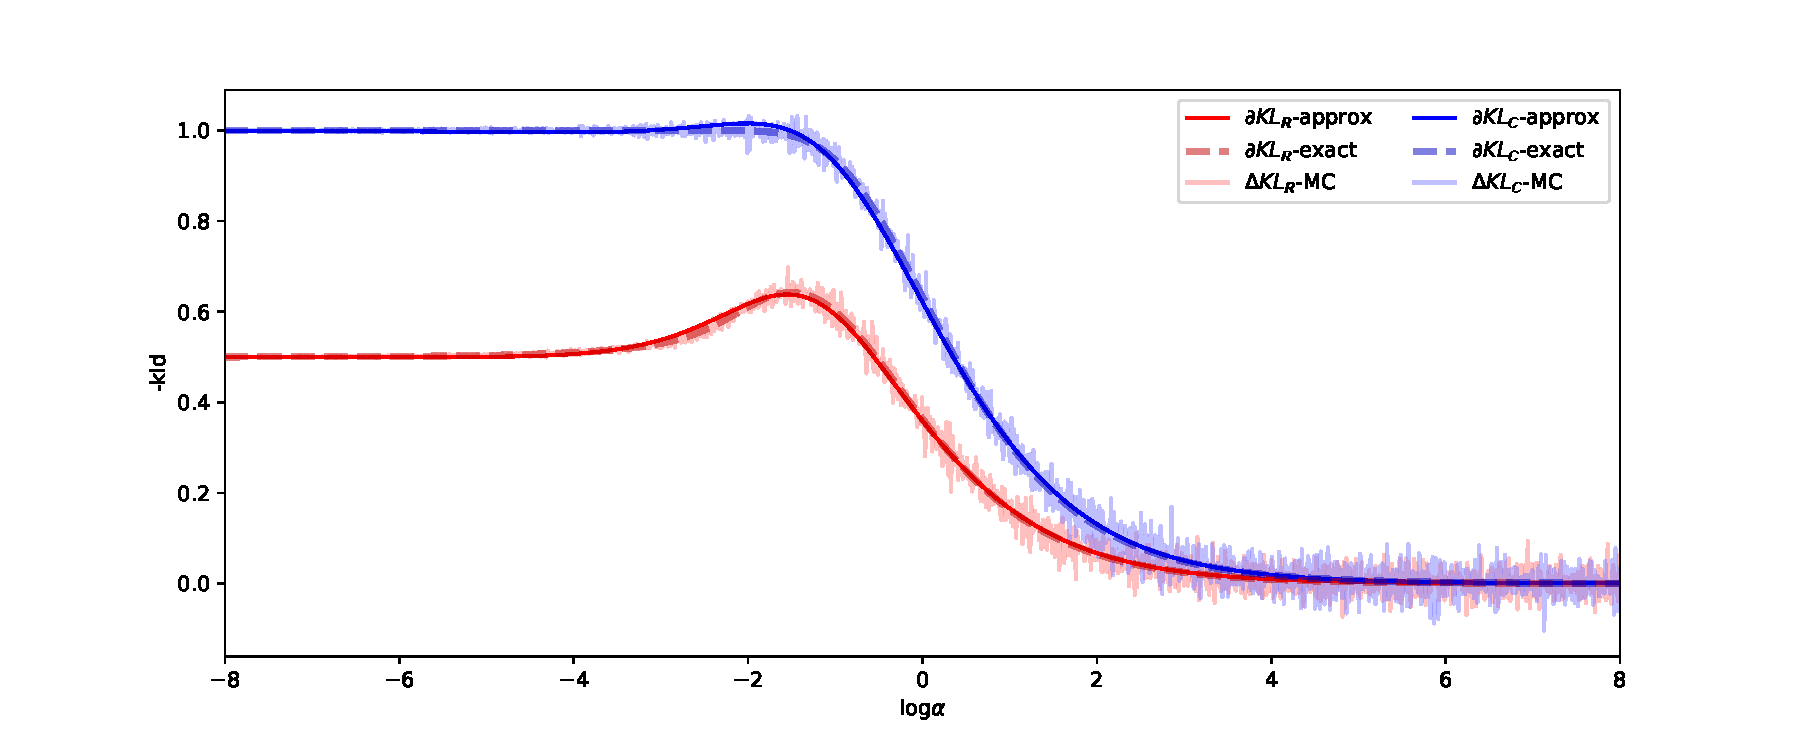
\includegraphics[width=1.\linewidth]{../notebooks/assets/grad_log.pdf}
  \caption{$\tfrac{d f(\alpha)}{d \log{\alpha}}$ of the fit \citep{molchanov_variational_2017},
  MC estimate, and exact derivative using \eqref{eq:real-kl-div-deriv-log}.}
  \label{fig:molchanov-derivative-replica}
\end{figure}

% subsection real-chisq-grad (end)

\subsection{Backpropagation through $\cplx$-networks} % (fold)
\label{sub:wirtinger_calculus}

% essential intro into Wirtinger calculus (CR)
% https://math.stackexchange.com/a/444493
Wirtinger ($\cplx\real$) calculus relies on the natural identification of $\cplx$ with $
  \real \times \real
$, and regards $
  f\colon \cplx \to \cplx
$ as an equivalent in algebraic sense function $F\colon \real^2 \to \cplx$ defined $
  f(z) = f(u + jv) = F(u, v)
$. Within this framework the differential of $f$ at $z = u + jv \in \cplx$ is
$$
df(z)
  = \frac{\partial f}{\partial z} dz
    + \frac{\partial f}{\partial \conj{z}} d\conj{z}
   % = \frac12\bigl(
   %    \frac{\partial}{\partial u}
   %    - j \frac{\partial}{\partial v}
   % \bigr) F (du - j dv)
   % + \frac12\bigl(
   %    \frac{\partial}{\partial u}
   %    + j \frac{\partial}{\partial v}
   % \bigr) F (du - j dv)
   % = \frac12 \bigl(
   %    \frac{\partial F}{\partial u} du - j \frac{\partial F}{\partial v} du
   %    + j \frac{\partial F}{\partial u} dv + \frac{\partial F}{\partial v} dv
   % \bigr)
   % + \frac12 \bigl(
   %    \frac{\partial F}{\partial u} du + j \frac{\partial F}{\partial v} du
   %    - j \frac{\partial F}{\partial u} dv + \frac{\partial F}{\partial v} dv
   % \bigr)
   = \frac{\partial F}{\partial u} du
     + \frac{\partial F}{\partial v} dv
   = dF(u, v)
  \,, $$
with formally defined derivatives $
  \tfrac{\partial}{\partial z}
    = \tfrac12 \bigl(
      \tfrac{\partial}{\partial u}
      - j \tfrac{\partial}{\partial v}
    \bigr)
$ and $
  \tfrac{\partial}{\partial \conj{z}}
    = \tfrac12 \bigl(
      \tfrac{\partial}{\partial u}
      + j \tfrac{\partial}{\partial v}
    \bigr)
$, and differentials $dz = du + j dv$ and $d\conj{z} = du - j dv$. This implies that the
complex argument and its conjugate are treated as independent variables. Cauchy-Riemann
conditions $
  -j \tfrac{\partial F}{\partial v} = \tfrac{\partial F}{\partial u}
$ scan be expressed as $
  \tfrac{\partial f}{\partial \conj{z}} = 0
$ in this notation. Thus $\cplx\real$ calculus subsumes the usual $\cplx$-calculus on
holomorphic functions, when $f(z)$, regarded as $f(z, \conj{z})$, is constant with respect
to $\conj{z}$. The usual rules of calculus, like chain and product rules, follow directly
from the definition of the operators, e.g.
$$
  \frac{\partial (f\circ g)}{\partial z}
    = \frac{\partial f(g(z))}{\partial g} \frac{\partial g(z)}{\partial z}
    + \frac{\partial f(g(z))}{\partial \conj{g}} \frac{\partial \conj{g(z)}}{\partial z}
    % = \nabla G \nabla F
  \,. $$
% Show that $dh(z) = df(g(z)) dg(z)$.
% $h(z) = f(g(z)) = F(G_r(u, v), G_i(u, v)) = H(u, v)$
% $$
% dH
%   = \tfrac{\partial F}{\partial x} \tfrac{\partial G_r}{\partial u} du
%   + \tfrac{\partial F}{\partial x} \tfrac{\partial G_r}{\partial v} dv
%   + \tfrac{\partial F}{\partial y} \tfrac{\partial G_i}{\partial u} du
%   + \tfrac{\partial F}{\partial y} \tfrac{\partial G_i}{\partial v} dv
%   = \tfrac{\partial F}{\partial r} d\Re g(z)
%   + \tfrac{\partial F}{\partial i} d\Im g(z)
%   = df(\Re g(z) + j\Im g(z)) d g(z)
%   = df(g(z)) d g(z)
%   \,. $$

In machine learning tasks the target objective is typically empirical risk, which has to
be real-valued to be minimized. Nevertheless, the expression of the $\cplx\real$ gradient
is compatible with what is expected, when $f$ is treated like a $\real^2$ function. For a
real-valued $f\colon \cplx \to \real$ we have $\conj{f} = f$, which implies $
  \tfrac{\partial f}{\partial \conj{z}}
    = \tfrac{\partial \conj{f}}{\partial \conj{z}}
    = \conj{\tfrac{\partial f}{\partial z}}
$, whence
$$
df
  = \tfrac{\partial f}{\partial z} dz
    + \tfrac{\partial f}{\partial \conj{z}} d\conj{z}
  % = \conj{\tfrac{\partial \conj{f}}{\partial \conj{z}}} dz
  % + \conj{\conj{\tfrac{\partial f}{\partial \conj{z}}} dz}
  = 2 \Re \Bigl(
    \conj{\tfrac{\partial f}{\partial \conj{z}}} dz
  \Bigr)
  = 2 \Re \bigl(
    \tfrac{\partial f}{\partial z} dz
  \bigr)
  \,. $$
Thus, the gradient of $f$ at $z$ is given by $
  \nabla_z f(z)
    = \tfrac{\partial F}{\partial u}
      + j \tfrac{\partial F}{\partial v}
$.

Natural identification of $\cplx$ with $\real\times \real$, storing the real and imaginary
parts in interleaved format, emulation of $\cplx$-algebra using $\real$-valued arithmetic,
and Wirtinger calculus make it possible to reuse $\real$-backpropagation and existing
auto-differentiation frameworks, \citep{trabelsi_deep_2017}.

% subsection wirtinger_calculus (end)

\subsection{$\cplx$-Linear operator representation} % (fold)
\label{sub:c-linear_operator_representation}

% proof that such operators exist and are unique (well this is an obvious statement)
Consider $L \colon \cplx^m \to \cplx^n$ -- linear in $\cplx$. Then $
  L(u + jv) = L u + j L v
$ for any $u, v \in \real^m$, which implies that the effect of $L$ as $\cplx$-linear
operator is determined by its restriction onto $\real^n$. Let $
  F = L\vert_{\real^m}
  \colon \real^m \to \cplx^n
$ and observe that $F_r = \Re \circ F$ and $F_i = \Im \circ F$ are $\real$-linear operators
such that $F = F_r + j F_i$ (pointwise). Indeed,
$$
  F_r(a + \lambda b)
  % = \Re F(a + \lambda b)
  = \Re L(a + \lambda b)
  % = \Re \bigl( L a + \lambda L b \bigr)
  = \Re L a + \lambda \Re L b
  % = \Re F a + \lambda \Re F b
  = F_r a + \lambda F_r b
  \,. $$
Therefore for any $\cplx$-linear operator $L$ there are $\real$-linear operators $U, V$
such that
$$
L z 
  = (U + j V) (\Re z + j \Im z)
  % = (U + j V) \Re z + j (U + j V) \Im z
  % = U \Re z + j V \Re z + j \bigl(U \Im z + j V \Im z \bigr)
  = U \Re z - V \Im z + j \bigl( V \Re z + U \Im z \bigr)
  % = (U + j V) z
  \,. $$
Uniqueness of these operators follows, if this decomposition is applied to any $z$ with
$\Im z = 0$.

% subsection c-linear_operator_representation (end)

\subsubsection{MGF of a noncentral $\chi^2$} % (fold)
\label{ssub:mgf_of_a_noncentral_chi}

Consider the mgf of $W$:
$$
M_W(t)
  = \mathbb{E}(e^{Wt})
  = \prod_i \mathbb{E}(e^{(\mu_i + z_i)^2 t})
  \,, $$
by independence. Now for $z \sim \mathcal{N}(\mu, 1)$
$$
\mathbb{E}(e^{z^2 t})
  = \tfrac1{\sqrt{2\pi}}
  \int_{-\infty}^{+\infty}
      e^{z^2 t} e^{-\tfrac{(z-\mu)^2}2}
  dz
  \,. $$
Now, for $t < \tfrac12$
$$
z^2 t - \tfrac{(z - \mu)^2}2
  = - \tfrac12 (1 - 2t) z^2 + z \mu - \tfrac{\mu^2}2
  % = - \tfrac12 (1 - 2t) \bigl(
  %   z^2 - 2 z \tfrac\mu{1 - 2t} + \tfrac{\mu^2}{1 - 2t}
  % \bigr)
  % = - \tfrac12 (1 - 2t) \bigl( z - \tfrac\mu{1 - 2t} \bigr)^2
  % - \tfrac12 (1 - 2t) \bigl(
  %   \tfrac{\mu^2}{1 - 2t}
  %   - \tfrac{\mu^2}{(1 - 2t)^2}
  % \bigr)
  % = - \tfrac12 (1 - 2t) \bigl( z - \tfrac\mu{1 - 2t} \bigr)^2
  %   - \tfrac{\mu^2}2 \bigl(
  %   \tfrac{1 - 2t}{1 - 2t} - \tfrac1{1 - 2t}
  % \bigr)
  % = - \tfrac12 (1 - 2t) \bigl( z - \tfrac\mu{1 - 2t} \bigr)^2
  %   + \tfrac{\mu^2}2 \tfrac{2t}{1 - 2t}
  = - \tfrac12 (1 - 2t) \bigl( z - \tfrac\mu{1 - 2t} \bigr)^2
    + \mu^2 \tfrac{t}{1 - 2t}
  \,, $$
whence
\begin{multline}
  \mathbb{E}(e^{z^2 t})
    = \tfrac1{\sqrt{2\pi}}
      \int_{-\infty}^{+\infty}
        e^{z^2 t} e^{-\tfrac{(z-\mu)^2}2}
      \, dz
    % = e^{\mu^2 \tfrac{t}{1 - 2t}}
    %   \tfrac1{\sqrt{2\pi}}
    %   \int_{-\infty}^{+\infty}
    %     e^{- \tfrac12 (1 - 2t) \bigl( z - \tfrac\mu{1 - 2t} \bigr)^2}
    %   \, dz
    \\= e^{\mu^2 \tfrac{t}{1 - 2t}}
      \tfrac1{\sqrt{2\pi}}
      \int_{-\infty}^{+\infty}
        e^{- \tfrac12 (1 - 2t) z^2}
      \, dz
    % = [u = \sqrt{1 - 2t} z]
    % = e^{\mu^2 \tfrac{t}{1 - 2t}}
    %   \tfrac1{\sqrt{2\pi}}
    %   \int_{-\infty}^{+\infty}
    %     e^{- \tfrac12 u^2}
    %   \, \tfrac{du}{\sqrt{1 - 2t}}
    = \tfrac{
        \exp{\{\mu^2 \tfrac{t}{1 - 2t}\}}
    }{\sqrt{1 - 2t}}
    \,.
\end{multline}
Therefore
$$
M_W(t)
  = \mathbb{E}(e^{Wt})
  = \prod_i \tfrac{
      e^{\mu_i^2 \tfrac{t}{1 - 2t}}
    }{\sqrt{1 - 2t}}
  % = e^{\lambda \tfrac{t}{1 - 2t}}
  %   (1 - 2t)^{-\tfrac{m}2}
  % = e^{\lambda \tfrac{- t}{2t - 1}}
  %   (1 - 2t)^{-\tfrac{m}2}
  % = e^{\tfrac\lambda2 \tfrac{1 - 2t - 1}{2t - 1}}
  %   (1 - 2t)^{-\tfrac{m}2}
  % = e^{- \tfrac\lambda2 (1 + \tfrac1{2t - 1})}
  %   (1 - 2t)^{-\tfrac{m}2} 
  = e^{- \tfrac\lambda2} e^{\tfrac\lambda2 \tfrac1{1 - 2t}}
  (1 - 2t)^{-\tfrac{m}2}
  \,. $$
Expanding the exponential as infinite series:
\begin{multline}
  M_W(t)
    = e^{- \tfrac\lambda2} e^{\tfrac\lambda2 \tfrac1{1 - 2t}}
    (1 - 2t)^{-\tfrac{m}2}
    % = e^{- \tfrac\lambda2} (1 - 2t)^{-\tfrac{m}2}
    %   \sum_{n \geq 0} \tfrac{\bigl(\tfrac\lambda2\bigr)^n}{n! (1 - 2t)^n}
    \\= \sum_{n \geq 0} \tfrac{e^{- \tfrac\lambda2} \bigl(\tfrac\lambda2\bigr)^n}{n!}
        (1 - 2t)^{-\tfrac{2n + m}2}
    = \sum_{n \geq 0} \tfrac{e^{- \tfrac\lambda2} \bigl(\tfrac\lambda2\bigr)^n}{n!}
        \mathbb{E}_{x \sim \chi^2_{m + 2n}}(e^{x t})
    \,.
\end{multline}

% subsubsection mgf_of_a_noncentral_chi (end)

% section appendix (end)

\end{document}